\documentclass{llncs}
\usepackage{algorithm}
\usepackage{algpseudocode}
\usepackage{fixltx2e}
\usepackage{subcaption}
\captionsetup{compatibility=false}
\usepackage{amsmath}
\usepackage{mathtools}
\usepackage{tikz}
\usetikzlibrary{trees}
\usetikzlibrary{positioning}

\algnewcommand{\IIf}[1]{\State\algorithmicif\ #1\ \algorithmicthen}
\algnewcommand{\EndIIf}{}
\algnewcommand{\IfElse}[3]{\algorithmicif\ #1\ \algorithmicthen\ #2\ \algorithmicelse\ #3}
\algnewcommand{\EndIfElse}{}
\MakeRobust{\Call}
\newcommand{\True}{\texttt{true}}
\newcommand{\False}{\texttt{false}}
\newcommand{\II}{\mathcal{I}}
\newcommand{\textoverline}[1]{$\overline{\mbox{#1}}$}

\pagestyle{headings}

\begin{document}

\title{A SAT-Based Counterexample Guided Method for Unbounded Synthesis}

\author{}
\institute{}

%\author{Alexander Legg\inst{1} 
%    \and Nina Narodytska\inst{2}
%    \and Leonid Ryzhyk\inst{2}}
%
%\institute{NICTA\thanks{NICTA is funded by the Australian Government as represented by the Department of Broadband,
%    Communications and the Digital Economy and the Australian Research Council through the ICT
%    Centre of Excellence program.} and UNSW \\
%    \email{alexander.legg@nicta.com.au}
%    \and Samsung Research America}

\maketitle

\sloppy

\begin{abstract}

    Reactive synthesis techniques based on constructing the winning region of
    the system have been shown to work well in many cases but suffer from state
    explosion in others.  A different approach, proposed recently, applies SAT
    solvers in a counterexample guided framework to solve the synthesis
    problem.  However, this method is limited to synthesising systems that
    execute for a bounded number of steps and is incomplete for synthesis with
    unbounded safety and reachability objectives.  We present an extension of
    this technique to unbounded synthesis.  Our method applies Craig
    interpolation to abstract game trees produced by counterexample-guided
    search in order to construct a monotonic sequence of may-losing regions.
    Experimental results based on SYNTCOMP 2015 competition benchmarks show
    this to be a promising alternative that solves some previously intractable
    instances.

\end{abstract}

\section{Introduction}

Reactive systems are ubiquitous in real-world problems such as circuit design,
industrial automation, or device drivers. Automatic synthesis can provide a
\emph{correct by construction} controller for a reactive system from a
specification.  However, the reactive synthesis problem is 2EXPTIME-complete so
naive algorithms are infeasible on anything but simple systems.

Reactive synthesis is formalised as a game between the \emph{controller} and
its \emph{environment}. In this work we focus on safety games, in which the
controller must prevent the environment from forcing the game into an error
state. In this way the environment is equivalent to an existential search of
the game and the controller is universal. Much of the complexity of reactive
synthesis stems from managing the interactions of the alternating quantifiers
on the state space of the game.

There are several techniques that aim to mitigate this complexity by
representing states symbolically.  Historically the most successful technique
has been to use \emph{Binary Decision Diagrams} (BDDs).  BDDs efficiently
represent a relation on a set of game variables but in the worst case the
representation may be exponential in the number of variables. This means that
BDDs are not a one-size-fits-all solution for all reactive synthesis
specifications.

Advances in SAT solving technology has prompted research into its applicability
to synthesis as an alternative to BDDs. One approach is to find sets of states
in CNF \cite{bloem2014,morgenstern2013}. Another approach is to eschew states
and focus on \emph{runs} of the game. Previous work has applied this idea to
realizability of bounded games \cite{narodytska2014} by forming abstractions of
the game and refining in a counterexample-guided framework. This has been shown
to outperform BDDs on certain classes of game specifications but is only able
to find counterexamples of a certain length to the safety property.  In this
paper, we extend this idea to unbounded games by approximating sets of unsafe
states from abstract games. Careful construction ensures that a fixed point in
these sets guarantees completeness.

Section 2 outlines the original bounded synthesis algorithm. In Section 3 we
describe and prove the correctness of our extension of the algorithm to
unbounded games. In the following sections we discuss optimisations to the
algorithm, evaluate our methodology, and compare our approach to other
synthesis techniques.

\section{Background}

A \emph{safety game}, $G = \langle X, L_u, L_c, \delta, I, E \rangle$,
is defined over boolean state variables $X$, uncontrollable label variables $L_u$, and
controllable label variables $L_c$.  $I$ is the initial state of the game given as a 
valuation of state variables.  $E(X)$ is the set of error states represented by its 
characteristic formula.  The transition relation $\delta(X, L_u, L_c, X')$ of the game 
is a boolean formula that relates current state and label to the set of possible next 
states of the game.  We assume deterministic games, where 
$\delta(x,u,c,x'_1) \land \delta(x,u,c,x'_2) \implies (x'_1=x'_2)$.


At every round of the game, the \emph{environment} picks an
uncontrollable label, the \emph{controller} responds by choosing a controllable 
label and the game transitions into a new state according to $\delta$. 
A \emph{run} of a game $(x_0, u_0, c_0), (x_1, u_1, c_1) \dots (x_n, u_n,
c_n)$ is a chain of state and label pairs s.t.\,$\delta(x_k, u_k, c_k, x_{k+1})$. 
A run is winning for the controller if $x_0 = I \land \forall i \in \{1..n\} (\lnot E(x_i))$. 
In a \emph{bounded game} of rank $n$ all runs are restricted to length $n$, whereas unbounded 
games consider runs of infinite length. Since we consider only deterministic games, a run 
is uniquely described by a list of assignments to $L_u$ and $L_c$.

A \emph{controller strategy} $\pi^c : (X, L_u) \to L_c$ is a mapping of states
and uncontrollable inputs to controllable labels. A controller strategy is
winning in a bounded game of rank $n$ if all runs $(x_0, u_0, \pi^c(x_0, u_0)),
(x_1, u_1, \pi^c(x_1, u_1)) \dots$ $(x_n, u_n, \pi^c(x_n, u_n))$ are winning.
Bounded \emph{realizability} is the problem of determining the existence of
such a strategy for a bounded game.

An \emph{environment strategy} $\pi^e : X \to L_u$ is a mapping of states to
uncontrollable labels. A bounded run is winning for the environment if $x_0
= I \land \exists i \in \{1..n\} (E(x_i))$ and an environment strategy is
winning for a bounded game if all runs $(x_0, \pi^e(x_1), c_1), (x_1,
\pi^e(x_1), c_1) \dots (x_n, \pi^e(x_n), c_n)$ are winning for the environment.
Safety games are zero sum, therefore the existence of a winning controller strategy
implies the nonexistence of a winning environment strategy and vice versa.

\subsection{Realisability of Bounded Safety Games}

We review the bounded synthesis algorithm by Narodytska et
al.~\cite{narodytska2014}, which is the main building block for our unbounded
algorithm.

Realisability for a bounded safety game can be solved by checking an
quantified formula consisting of the game's transition relation \emph{unrolled}
to the length of the bounded game. The quantifiers represent the two players of
the game: universal for the controller and existential for the environment.
Just as the players alternate in choosing actions every step of the game, there
must be quantifier alternations in the formula for each unrolling.

Instead of solving both quantifiers at once, two competing solvers are used to
solve abstractions of the game. Each solver builds a candidate strategy for its
corresponding player and uses its opponent's candidate to restrict its own
search. The solvers communicate to refine one another's candidate strategies by
finding counterexamples. Eventually one solver will be unable to find a
counterexample indicating that its opponent's candidate strategy is a winning
strategy for the game.

\subsection{Abstract Game Trees}

\tikzset{every node/.style={solid}}
\tikzstyle{fixed}=[solid]
\tikzstyle{unfixed}=[dash pattern = on 2pt off 2pt]
\begin{figure}
    \centering
    \begin{subfigure}[t]{.25\textwidth}
        \centering
        \begin{tikzpicture}[dash pattern = on 2pt off 2pt, level distance = 10mm]
            \node [circle,draw] (root){}
                child {node [circle,draw] {}
                    child {node [circle,draw] {}
                        edge from parent [fixed] node [left] {$b$}
                    }
                    edge from parent [fixed] node [left] {$a$}
                }
                child {node [circle,draw] {}
                    edge from parent [fixed] node [right] {$d$}
                }
                node [above=4pt] {$\langle s, k \rangle$};
        \end{tikzpicture}
        \captionsetup{width=.8\textwidth}
        \caption{AGT}
        \label{fig:agt}
    \end{subfigure}%
    \begin{subfigure}[t]{.25\textwidth}
        \centering
        \begin{tikzpicture}[dash pattern = on 2pt off 2pt, level distance = 10mm]
            \node [circle,draw] (root){}
                child {node [circle,draw] {}
                    child {node [circle,draw] {}
                        node [left=4pt] {$\epsilon$}
                        edge from parent [fixed] node [left] {$b$}
                    }
                    node [left=4pt] {$\beta$}
                    edge from parent [fixed] node [left] {$a$}
                }
                child {node [circle,draw] {}
                    node [left=4pt] {$\gamma$}
                    edge from parent [fixed] node [right] {$d$}
                }
                node [right=4pt] {$\alpha$}
                node [above=4pt] {$\langle s, k \rangle$};
        \end{tikzpicture}
        \captionsetup{width=.8\textwidth}
        \caption{AGT with strategy}
        \label{fig:strategy}
    \end{subfigure}%
    \begin{subfigure}[t]{.25\textwidth}
        \centering
        \begin{tikzpicture}[dash pattern = on 2pt off 2pt, level distance = 10mm]
            \node [circle,draw] (root){}
                child {node [circle,draw] {}
                    child {node [circle,draw] {}
                        node [left=4pt] {$\epsilon$}
                        edge from parent [fixed] node [left] {$b$}
                    }
                    node [left=4pt] {$\beta$}
                    edge from parent [fixed] node [left] {$a$}
                }
                child {node [circle,draw] (sroot) {}
                    child {node [below left=0 and -10pt] (sa) {}
                        edge from parent [draw=none]
                    }
                    child {node [below right=0 and -10pt] (sb) {}
                        edge from parent [draw=none]
                    }
                    node [left=4pt] {$\gamma$}
                    edge from parent [fixed] node [right] {$d$}
                }
                node [right=4pt] {$\alpha$}
                node [above=4pt] {$\langle s, k \rangle$};
                \draw[unfixed] (sa.center) -- (sb.center);
                \draw[unfixed] (sroot.south) -- (sa.center);
                \draw[unfixed] (sroot.south) -- (sb.center);
        \end{tikzpicture}
        \captionsetup{width=.8\textwidth}
        \caption{AGT with spoiling strategy}
        \label{fig:spoiling}
    \end{subfigure}%
    \begin{subfigure}[t]{.25\textwidth}
        \centering
        \begin{tikzpicture}[dash pattern = on 2pt off 2pt, level distance = 10mm]
            \node [circle,draw] (root){}
                child {node [circle,draw] {}
                    child {node [circle,draw] {}
                        edge from parent [fixed] node [left] {$b$}
                    }
                    edge from parent [fixed] node [left] {$a$}
                }
                child {node [circle,draw] {}
                    child {node [circle,draw] {}
                        edge from parent [fixed] node [right] {$e$}
                    }
                    edge from parent [fixed] node [right] {$d$}
                }
                node [above=4pt] {$\langle s, k \rangle$};
        \end{tikzpicture}
        \captionsetup{width=.8\textwidth}
        \caption{Refined AGT}
        \label{fig:refined}
    \end{subfigure}
    \caption{Abstract game trees}
    \label{fig:alltrees}
\end{figure}

An abstraction of the game restricts actions available to one of the players.
Specifically, we consider abstractions represented as trees of actions,
referred to as \emph{abstract game trees}.  Together with a state-round pair
$\langle s,k\rangle$, an abstract game tree defines an \emph{abstract game}
played from this state.  In the abstract game, the environment player is
required to pick actions from the tree, starting from the root node.  After
reaching a leaf, it continues playing unrestricted.  The tree in
Figure~\ref{fig:agt} restricts the initial environment action to the set $\{a,
d\}$.  After choosing action $d$, the environment reaches a leaf of the tree
and continues playing unrestricted.  Alternatively, after choosing $a$, the
environment is required to play action $b$ in the next round.  

Nodes of an abstract game tree are uniquely identified by the list of edge
labels along the path from the root to the node.  We identify an abstract game
tree with the set of its nodes.  For example, the tree in Figure~\ref{fig:agt}
can be written as $\{(),(d),(a),(a,b)\}$.  We denote $\textsc{leaves}(T)$ the
subset of leaf nodes of a tree $T$. 

A \emph{partial strategy} $Strat: T \rightarrow L_c $ assigns a controllable
action to be played in each node of the abstract game tree.
Figure~\ref{fig:strategy} shows an example partial strategy.  The controller
starts by choosing action $\alpha$.  If the environment plays $a$, the
controller responds with $\beta$ in the next round, and so on. Given a partial
strategy $Strat$, we can map each leaf $l$ of the abstract game tree to
$\langle s',i'\rangle=\textsc{outcome}(\langle s, i\rangle, Strat, l)$ obtained
by playing all controllable and uncontrollable actions on the path from the
root to the leaf.

\subsection{Counterexample-guided bounded synthesis}

The bounded synthesis algorithm solves abstract game trees by invoking a SAT
solver to search for candidate partial strategies. Candidate strategies are
checked and by a call to the opponent solver, which also refines the abstract
game tree. The refinements are then solved recursively.  The full procedure is
illustrated in Algorithm~\ref{alg:bounded}.

\begin{algorithm}
    \begin{algorithmic}[1]
        \Function{solveAbstract}{$p, \langle s, k \rangle , T$}
        \State $cand \gets $ \Call{findCandidate}{$p, \langle s, k \rangle, T$} \Comment{Look for a candidate}
        \IIf{$k = n - 1$} \Return $cand$ \EndIIf \Comment{Reached the bound}
        \State $T' \gets T$
        \Loop
            \IIf{$cand = \emptyset $} \Return $\emptyset $ \EndIIf \Comment{No candidate: return with no solution}
            \State $\langle cex, l, u \rangle \gets $ \Call{verify}{$p, \langle s, k \rangle, T, cand$} \Comment{Verify candidate}
            \IIf{$cex = \False$} \Return $cand$ \EndIIf \Comment{No counterexample: return candidate}
            \State $T' \gets $ \Call{gtAppend}{$T', l, u$} \Comment{Refine AGT with counterexample}
            \State $cand \gets $ \Call{solveAbstract}{$p, \langle s, k \rangle, T'$} \Comment{Solve refined AGT}
        \EndLoop
        \EndFunction
        \algstore{b1}
    \end{algorithmic}

    \begin{algorithmic}
        \algrestore{b1}
        \Function{findCandidate}{$p, \langle s, k \rangle, T$}
            \State $f \gets $ \IfElse{$p = \texttt{cont}$}{\Call{treeFormula}{$T$}}{\Call{\textoverline{treeFormula}}{$T$}} \EndIfElse
            \State $sol \gets $ \Call{SAT}{$s(X_T) \land f$}
            \If{$sol = \texttt{unsat}$} 
                \If{\texttt{unbounded}} \Comment{Active only in the unbounded solver}
                    \State $\sigma \gets $ \Call{generalise}{$s$} \Comment{Expand $s$ to a set of states}
                    \State \IfElse{$p = \texttt{cont}$}{\Call{learn}{$\sigma, T$}}{\Call{\textoverline{learn}}{$\sigma, T$}} \EndIfElse
                \EndIf
                \State \Return $\emptyset$ \Comment{No candidate exists}
            \Else
                \State \Return $\{ \langle n, c \rangle | n \in $ \Call{gtNodes}{T} $, c = \Call{sol}{n} \}$ \Comment{Fix candidate moves in $T$}
            \EndIf
        \EndFunction
        \algstore{b2}
    \end{algorithmic}

    \begin{algorithmic}
        \algrestore{b2}
        \Function{verify}{$p, \langle s, k\rangle, gt, cand$}
            \For{$l \in leaves(gt)$}
            \State $\langle k', s'\rangle \gets $ \Call{outcome}{$\langle s, k\rangle, gt, l$} \Comment{Get rank and state at leaf}
                \State $u \gets $ \Call{solveAbstract}{\Call{opponent}{$p$}, $\langle k', s' \rangle, \emptyset$} \Comment{Solve for the opponent}
                \IIf{$u \neq \emptyset$} \Return $\langle \False, l, u \rangle$ \EndIIf \Comment{Return counterexample}
            \EndFor
            \State \Return $\langle \True, \emptyset, \emptyset \rangle$
        \EndFunction
    \end{algorithmic}

    \caption{Bounded Synthesis}
    \label{alg:bounded}
\end{algorithm}
    
The algorithm takes a concrete game $G$ as an implicit argument. In addition it
takes a player (controller or environment), state-round pair $\langle s,
k\rangle$ and an abstract game tree $T$ and returns a winning partial strategy
for $T$, if one exists.  The environment takes the first move in each step of
the game so the algorithm initially plays on the environment's behalf. The
initial invocation takes the initial state $\langle I, n\rangle$ and an empty
abstract game tree $\emptyset$. The empty game tree does not constrain opponent
moves, hence solving such an abstraction is equivalent to solving the original
concrete game.

The algorithm is organised as a counterexample-guided abstraction refinement
(CEGAR) loop.  The first step of the algorithm uses the \textsc{findCandidate}
function, described in detail below, to come up with a candidate partial
strategy for $T$. If it fails to find a strategy, this means that no winning
partial strategy exists for $T$.  If, on the other hand, a candidate partial
strategy is found, we need to verify if it is indeed winning for $T$.

The \textsc{verify} procedure searches for a \emph{spoiling} counterexample
strategy in each leaf of the candidate partial strategy by calling
\textsc{solveAbstract} for the opponent. The dual solver solves games on behalf
of the controller player.  {Figure~\ref{fig:spoiling}} shows a spoiling
strategy discovered one of the leaves of the partial strategy.

If the dual solver can find no spoiling strategy at any of the leaves, then the
candidate partial strategy is a winning one. Otherwise, \textsc{verify} returns
the move used by the opponent to defeat a leaf of the partial strategy, which
is appended to the corresponding node in $T$ in order to refine it in line~(9)
as shown in Figure~(\ref{fig:refined}).

We solve the refined game by recursively invoking \textsc{solveAbstract} on it.
If no partial winning strategy is found for the refined game then there is also
no partial winning strategy for the original abstract game, and the algorithm
returns a failure.  Otherwise, the partial strategy for the refined game is
\emph{projected} on the original abstract game by removing the leaves
introduced by refinements. The resulting partial strategy becomes a candidate
strategy to be verified at the next iteration of the loop. In the worst case
the loop terminates after all actions in the game are refined into the abstract
game.

The way game trees are refined is determined by the formula passed to the SAT
solver in $\textsc{findCandidate}$. This formula contains CNF encodings of all
of the unrolled runs represented by an abstract game tree and the winning
condition of the current player. Runs are encoded by copying the transition
relation for every step in the abstract game. When playing for the controller,
the SAT solver searches for a satisfying assignment to the unfixed label
variables in tree so that none of the runs reaches the error state. The
environment formulation is satisfiable if any run does reach the error state.
The formula is constructed recursively from the root of a tree by
$\textsc{treeFormula}$.

Since the game tree formulation is passed to a SAT solver, both controllable
and uncontrollable unfixed labels will be existentially quantified. This means
that the SAT solver will find any way to win the game while both players are
cooperating. If no winning run exists in an abstract game even when the players
are cooperating then there is no winning run when the opponent is playing
adversarily. When a winning run is found, the actions chosen by the SAT solver
are used to refine the game tree. This is advantageous for many synthesis
problems where the game must be formalised as adversarial for correctness but
the final implementation will be cooperating with its environment in the real
world. An example of such a system is a device driver that cooperates with the
device and OS to interface between the two.

\begin{algorithm}
    \caption{Tree formulas for Controller and Environment respectively}
    \label{alg:treeFormula}
    \begin{algorithmic}[1]
        \Function{treeFormula}{$T$}
        \If{$\Call{rank}{T} = 0$}
        \State \Return{ $\lnot \Call{E}{X_{T}}$ }
        \Else
        \State \Return{$\lnot \Call{E}{X_{T}} \land$ \\
            $$\bigwedge_{n \in \Call{succ}{T}}(\Call{$\delta$}{X_n, U_n, C_n, X'_n} \land \Call{label}{n} \land \Call{treeFormula}{n})$$
        }
        \EndIf
        \EndFunction
        \algstore{tf1}
    \end{algorithmic}

    \begin{algorithmic}[1]
        \algrestore{tf1}
        \Function{\textoverline{treeFormula}}{$T$}
        \If{$\Call{rank}{T} = 0$}
        \State \Return{\Call{E}{$X_{T}$}}
        \Else
        \State \Return{ $\Call{E}{X_{T}} \lor$ \\
        $$\bigvee_{n \in \Call{succ}{T}}(\Call{$\delta$}{X_n, U_n, C_n, X'_n} \land \Call{label}{n} \land \Call{\textoverline{treeFormula}}{n})$$ }
        \EndIf
        \EndFunction
    \end{algorithmic}
\end{algorithm}

%%%The bounded synthesis algorithm (Algorithm \ref{alg:bounded}) begins with an
%%%empty game as seen in Figure \ref{fig:emptytree}.  Initially we are playing on
%%%behalf of the environment because it chooses the first move in each step.  The
%%%empty game is passed to the SAT solver, which searches for a candidate
%%%environment strategy.  If a candidate is found (Figure \ref{fig:candidate})
%%%then it is checked for a spoiling strategy by solving for the controller.  If
%%%no spoiling strategy exists, that means our candidate is a winning strategy and
%%%the algorithm terminates.  Otherwise we find a counterexample (Figure
%%%\ref{fig:cex}), which is used to refine the empty game tree to include the
%%%first move from the controller's spoiling strategy (Figure \ref{fig:refined}).
%%%The algorithm continues by finding a new candidate for the environment (Figure
%%%\ref{fig:candidate2}), and a new counterexample to refine the game abstraction
%%%once again (Figure \ref{fig:refined2}). The full procedure is listed in
%%%Algorithm \ref{alg:bounded}.


\section{Unbounded Synthesis}

\label{sect:unbounded}

Bounded synthesis can be used to prove the existence of a winning strategy for
the environment on the unbounded game by providing a witness. For the
controller, the strongest claim that can be made is that the strategy is
winning as long as the game does not extend beyond the bound.

It is possible to set a bound such that all runs in the unbounded game will be
considered. The na\"ive approach is to use size of the state space as the bound
($2^{|X|}$) so that all states may be explored by the algorithm. A more nuanced
approach is to use the diameter of the game \cite{biere1999}, which is the
smallest number $d$ such that for any state $x$ there is a path of length $\leq
d$ to all other reachable states. This approach is common in bounded model
checking but for synthesis it quickly becomes intractable to consider such long
runs.

When performing model checking or synthesis with BDDs \cite{burch1990} the set
of states that are winning for the environment is iteratively constructed by
computing the states from which the environment can force the game into the
previous winning set. Eventually this process reaches a fixed point and the
total set of environment winning states is known.

A similar concept can be applied to the bounded synthesis algorithm to
iteratively increase the bound of the game and terminate when a fixed point is
reached. When a strategy is found to be winning on an abstract game tree, we
record as winning the states from which the opponent could find no
counterexample. To find these states we use interpolation of subformulas of the
game tree.


\subsection{Extending Bounded Synthesis to Unbounded Games}

\begin{algorithm}[h]
    \begin{algorithmic}[1]
        \Function{solveUnbounded}{$T$}
            \State $B^M \gets E$
            \State $B^m[0] \gets E$
            \For{$k = 1 \dots$}
                \IIf{\Call{SAT}{$I \land B^M$}}
                    \Return \texttt{unrealisable} \Comment{Losing in the initial state}
                \EndIIf
                \IIf{$\exists i \  B^m[i] \equiv B^m[i+1]$}
                    \Return \texttt{realisable} \Comment{Reached fixed point}
                \EndIIf
                \State $B^m[k] \gets \top$
                \State \Call{checkRank}{$I, k$}
            \EndFor
        \EndFunction
        \algstore{u1}
    \end{algorithmic}

    \begin{algorithmic}
        \algrestore{u1}
        \Require \emph{May} and \emph{must} invariants hold
        \Ensure \emph{May} and \emph{must} invariants hold
        \Ensure $\lnot s \in B^m[k]$ if there is a winning controller strategy of length $k$ starting at $s$
        \Ensure $s \in B^M$ if there is a winning environment strategy of length $k$ starting at $s$
%%%        $\exists u_{k..1} \forall c_{k..1} \  s(x_k) \land (E_k \lor (\delta(x_k, u_k, c_k) \land E(x_{k-1}) \lor ... \land E(x_1) \lor (\delta(x_1, u_1, c_1) \land E(x_0))...)$
%%%            $\forall u_{k..1} \exists c_{k..1} \  s(x_k) \land \lnot E_k \land \delta(x_k, u_k, c_k) \land \lnot E(x_{k-1}) \land ... \land \delta(x_1, u_1, c_1) \land \lnot E(x_0)$
        \Function{checkRank}{$s, k$}
            \State \Return \Call{solveAbstract}{$\texttt{env}, \langle s, k \rangle, \emptyset$}
        \EndFunction
    \end{algorithmic}
    \caption{Unbounded Synthesis}
    \label{alg:unbounded}
\end{algorithm}

The unbounded synthesis algorithm (Algorithm \ref{alg:unbounded}) effectively
consists of two communicating solvers: the counterexample-guided bounded
reachability solver and the unbounded solver based on incremental induction.
The unbounded solver calls the bounded solver with an increasing bound (line 8)
while learning states from abstract game trees that either must or may lose for
the controller. When the initial state is contained within the must-losing
states the game is known to be unrealisable (line 5).

May-losing states are learned by removing controller-winning states. We
maintain a set of states for every rank up the current bound. The states we
learn while executing the bounded algorithm can only said to be
controller-winning for a particular rank or below. However, we construct each
set carefully such that it is monotonically larger than the set of the rank
below (see Figure \ref{fig:maylosing}) and so that the environment is unable to
force play from one set to the next. Due to this careful construction, when two
adjacent sets become equivalent we know that the algorithm has reached a fixed
point and the controller is winning in the unbounded game (line 6).

\begin{figure}
    \centering
    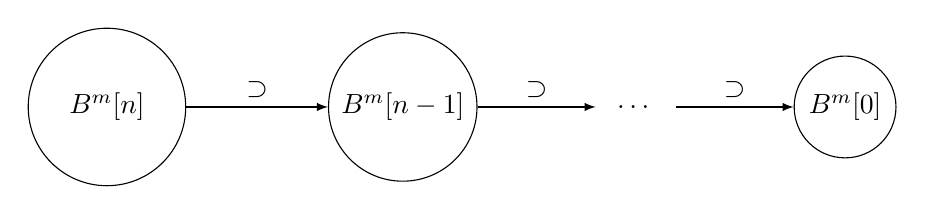
\begin{tikzpicture}
        \node [minimum size=2cm,circle,draw] (a){$B^m[n]$};
        \node [minimum size=1.5cm,circle,draw,right=1.8cm of a] (b){$B^m[n-1]$};
        \node [minimum size=1cm,right=1.5cm of b] (dots){$\dots$};
        \node [minimum size=0.5cm,circle,draw,right=1.5cm of dots] (c){$B^m[0]$};
        \draw[-latex] (a.east) -- node [above] {$\supset$} (b.west);
        \draw[-latex] (b.east) -- node [above] {$\supset$} (dots);
        \draw[-latex] (dots.east) -- node [above] {$\supset$} (c.west);
    \end{tikzpicture}
    \caption{May-losing states}
    \label{fig:maylosing}
\end{figure}


When executing the unbounded solver, lines 18 and 19 become active in the
bounded solver. These lines call the learning procedures when the solver fails
to find a candidate for an abstract game tree. The states symbolically
represented by nodes in the tree are losing for whichever player could not find
a winning candidate and can be extracted from the tree using interpolation.

\subsection{Learning States with Interpolants}

Given two formulas $A$ and $B$ such that $A \land B$ is unsatisfiable, it is
possible to construct a Craig interpolant\cite{craig1957} $\mathcal{I}$ such
that $A \to \mathcal{I}$, $B \land \mathcal{I}$ is unsatisfiable, and
$\mathcal{I}$ refers only to the intersection of variables in $A$ and $B$.  An
interpolant can be constructed efficiently from a resolution proof of the
unsatisfiability of $A \land B$ \cite{pudlak1997}.

\begin{figure}
    \centering
    \begin{tikzpicture}[dash pattern = on 2pt off 2pt, level distance = 10mm]
        \node [] (root){}
            child {node [circle,draw,label=left:$x_1$] {}
                child {node [circle,draw] {}
                    child {node [circle,draw,label=left:$x_0^0$] {} edge from parent[unfixed]}
                    edge from parent [fixed] node [left] {$u_1$}
                }
                child {node [circle,draw] {} edge from parent[unfixed]
                    child {node [circle,draw,label=right:$x_0^1$] {} edge from parent[unfixed]}
                    edge from parent [fixed] node [right] {$u_2$}
                }
                edge from parent [unfixed]
            };
    \end{tikzpicture}
%%%    \begin{tikzpicture}[overlay]
%%%        \draw [rotate = -20] (-1.9,0.35) ellipse (0.7 and 1.3);
%%%    \end{tikzpicture}
    \caption{A controller-losing game tree}
    \label{fig:interpolatetree}
\end{figure}

Consider the snippet of a game tree in Figure \ref{fig:interpolatetree}. The
tree is losing for the controller, the node labelled $x_1$ is at rank 1, and
$x_0^0$ and $x_0^1$ are at rank 0. Since the tree is controller-losing we know
that at least one run represented by the tree contains the error state.  As
a result, $\textsc{treeFormula}(gt)$ is unsatisfiable. If we take the step
$x_1$ to $x_0^0$ and cut it from the rest of the tree then
$\textsc{treeFormula}(step) \land \textsc{treeFormula}(parent)$ must too be
unsatisfiable.

We can construct an interpolant with $A = \textsc{treeFormula}(parent)$ and $B
= \textsc{treeFormula}(step)$. The only variables shared between $A$ and $B$
are the state variables at $x_1$. We know that $B \land \mathcal{I}$ is
unsatisfiable, therefore all states in $\mathcal{I}$ must lose to the
uncontrollable label $u_1$. We also know that $A \to \mathcal{I}$, thus
$\mathcal{I}$ contains all states reachable by the parent tree (on runs that
avoid the error state.)

\begin{algorithm}
    \caption{Amended tree formulas for Controller and Environment respectively}
    \label{alg:unboundedTreeFormula}
    \begin{algorithmic}[1]
        \Function{treeFormula}{gt}
        \If{$\Call{rank}{gt} = 0$}
        \State \Return{ $\lnot \Call{$B^M$}{x^{gt}}$ }
        \Else
        \State \Return{ $\lnot \Call{$B^M$}{x^{gt}} \land \bigwedge_{n \in \Call{succ}{gt}}(\Call{$\delta$}{n} \land \Call{label}{n} \land \Call{treeFormula}{n})$ }
        \EndIf
        \EndFunction
        \algstore{tf2}
    \end{algorithmic}

    \begin{algorithmic}
        \algrestore{tf2}
        \Function{\textoverline{treeFormula}}{gt}
        \If{$\Call{rank}{gt} = 0$}
        \State \Return{\Call{E}{$x^{gt}$}}
        \Else
        \State \Return{ $\Call{$B^m[rank(gt)]$}{x^{gt}} \land$ \\
            $(\Call{E}{x^{gt}} \lor \bigvee_{n \in \Call{succ}{gt}}(\Call{$\delta$}{n} \land \Call{label}{n} \land \Call{$\overline{treeFormula}$}{n}))$ }
        \EndIf
        \EndFunction
    \end{algorithmic}
\end{algorithm}

Now we can consider the step $x_1$ to $x_0^1$, and the parent - now without
either $x_1 \to x_0^0$ or $x_1 \to x_0^1$. The formula
$(\textsc{treeFormula}(parent) \land \mathcal{I}) \land
\textsc{treeFormula}(step)$ must be unsatisfiable. $\mathcal{I}$ contains all
states that lose to $u_1$ so any other state reachable at $x_1$ must lose to
$u_2$. Therefore we can compute another interpolant that contains states that
lose to $u_2$.

This is the foundation for a recursive algorithm that consumes an entire tree
by removing a single step on each iteration (Algorithm \ref{alg:learn}). All
learned states from which the controller \emph{must} lose are recorded in a set
of \emph{bad} states $B^M$.  This algorithm can also be performed on
environment-losing trees with the caveat that any state learnt at a node of
rank $n$ is only known to lose at ranks less than or equal to $n$. We negate
the interpolants we learn this way and record them in a mapping of ranks to
sets of states $B^m$ which \emph{may} be bad states for the controller.

\subsection{Correctness}

\begin{algorithm}
    \begin{algorithmic}[1]
        \Require $\sigma(X_T) \land $ \Call{treeFormula}{$T$} $\equiv \bot$
        \Require \emph{Must-invariant} holds
        \Ensure \emph{Must-invariant} holds
        \Ensure $\sigma(X_T) \land B^M$
        \Function{learn}{$\sigma, T$}
            \IIf{$T = \emptyset$}
                \Return
            \EndIIf
            \State $n \gets $ non-leaf node with max rank
            \State $\langle T_1, T_2 \rangle \gets $ \Call{gtSplit}{$T, n$}
            \State $\mathcal{I} \gets $ \Call{interpolate}{$\sigma(X_T) \land $ \Call{treeFormula}{$T_1$}, \Call{treeFormula}{$T_2$}}
            \State $B^M \gets B^M \lor \mathcal{I}$
            \State \Call{learn}{$\sigma, T_1$}
        \EndFunction
        \algstore{learn}
    \end{algorithmic}
    
    \begin{algorithmic}[1]
        \algrestore{learn}
        \Require $\sigma(X_T) \land $ \Call{\textoverline{treeFormula}}{$T$} $\equiv \bot$
        \Require \emph{May-invariant} holds
        \Ensure \emph{May-invariant} holds
        \Ensure $\sigma(X_T) \land B^m[$\Call{rank}{$T$}$] \equiv \bot$
        \Function{\textoverline{learn}}{$\sigma, T$}
            \IIf{$T = \emptyset$}
                \Return
            \EndIIf
            \State $n \gets $ non-leaf node with max rank
            \State $\langle T_1, T_2 \rangle \gets $ \Call{gtSplit}{$T, n$}
            \State $\mathcal{I} \gets $ \Call{interpolate}{$\sigma(X_T) \land $ \Call{\textoverline{treeFormula}}{$T_1$}, \Call{\textoverline{treeFormula}}{$T_2$}}
            \For{$i = 1$ to \Call{rank}{$n$}}
                \State $B^m[i] \gets B^m[i] \land \lnot \mathcal{I}$
            \EndFor
            \State \Call{\textoverline{learn}}{$\sigma, T_1$}
        \EndFunction
    \end{algorithmic}
    \caption{Learning algorithms}
    \label{alg:learn}
\end{algorithm}

The correctness of the unbounded synthesis algorithm can be established
independently from that of the bounded algorithm. Fortunately, the correctness
of the bounded solver has been established in \cite{narodytska2014}.

We define two global invariants of the algorithm.  The \emph{may-invariant}
states that sets $B^m[i]$ grows monotonically with $i$ and that each $B^m[i+1]$
overapproximates the uncontrollable predecessor of $f^m[i]$: $$\forall
i<k.~B^m[i] \subseteq B^m[i+1], Upre(B^m[i]) \subseteq B^m[i+1].$$

The \emph{must-invariant} guarantees that the must-losing set $B^M$ is an
underapproximation of the actual losing set $B$: $$B^M \subseteq B.$$

The sets $B^m$ and $B^M$ are only modified by the inductive solver, implemented
by \textsc{learn} and \textoverline{\textsc{learn}} functions.  Below we prove that these
functions indeed maintain the invariants.

\subsection{Proof of \textsc{\textoverline{learn}}}

We prove that postconditions of \textsc{\textoverline{learn}} are satisfied
assuming that its preconditions hold.

Line~(11) splits the tree $T$ into $T_1$ and $T_2$, such that $T_2$ has depth
1.  Consider formulas $f_1=\sigma(X_T) \land
\textsc{\textoverline{treeFormula}}(T_1)$ and $F_2 =
\textsc{\textoverline{treeFormula}}(T_2)$.  These formulas only share variables
$X_n$.  Their conjunction $F_1 \land F_2$ is unsatisfiable, as by construction
any solution of $F_1 \land F_2$ also satisfies $\sigma(X_T) \land
\textsc{treeFormula}(T)$, which is unsatisfiable (precondition (b)).  Hence the
interpolation operation is defined for $F_1$ and $F_2$.  

Intuitively, the interpolant computed in line~(13) overapproximates the set of
states reachable from $\sigma$ by following the tree from the root node to $n$,
and underapproximates the set of states from which the environment loses
against tree $T_2$.  

Formally, $\II$ has the property $\II \land F_2 \equiv \bot$.  Since $T_2$ is
of depth 1, this means that the environment cannot force the game into
$B^m[\textsc{rank}(n)]$ playing against the counterexample moves in $T_2$.
Hence, $\II \cap Upre(B^m[\textsc{rank}(n)]) = \emptyset$.  Furthermore, since
the may-invariant holds, $\II \cap Upre(i) = \emptyset$, for all $i <
\textsc{rank}(n)$.  Hence, removing $\II$ from all $B^m[i], i\leq
\textsc{rank}(n)$ in line~(15) preserves the may-invariant, thus satisfying the
first post-condition.

Furthermore, the interpolant satisfies $F_1 \rightarrow \II$, i.e., any
assignment to $X_n$ that satisfies $\sigma(X_T) \land
\textsc{\textoverline{treeFormula}}(T_1)$ also satisfies $\II$.  Hence,
removing $\II$ from $B^m[\textsc{rank}(n)]$ makes $\sigma(X_T) \land
\textsc{\textoverline{treeFormula}}(T_1)$ unsatisfiable, and hence all
preconditions of the recursive invocation of \textsc{\textoverline{learn}} in
line~(17) are satisfied.  

At the second last recursive call to \textsc{\textoverline{learn}}, tree $T_1$
is empty, $n$ is the root node, $\textsc{\textoverline{treeFormula}}(T_1)
\equiv B^m[\textsc{rank}(T)](X^T)$; hence $\sigma(X_T) \land
\textsc{\textoverline{treeFormula}}(T_1) \equiv \sigma(X_T) \land
B^m[\textsc{rank}(T)](X^T) \equiv \bot$.  Thus the second postcondition of
\textsc{\textoverline{learn}} holds.

\subsection{Proof of Termination}

We must prove that \textsc{checkRank} terminates and that upon termination its
postcondition holds.

We must prove that $\textsc{checkRank}$ terminates and that upon termination
its postcondition holds, i.e., state $s$ is removed from $B^m[k]$ if there is a
winning controller strategy on the bounded safety game of rank $k$ or it is
added to $B^M$ otherwise. Termination follows from completeness of
counterexample-guided search, which terminates after enumerating all possible
opponent moves in the worst case.

Assume that there is a winning strategy for the controller at rank $k$. This
means that at some point the algorithm discovers a counterexample tree of rank
$k$ for which the environment cannot force into $E$. The algorithm then invokes
the \textsc{\textoverline{learn}} method, adds $s$ to $B^M$.  Alternatively, if
there is a winning strategy for the environment at rank $k$ then a
counterexample losing for the controller will be found. Subsequently
\textsc{learn} will be called and $s$ eliminated from $B^m[k]$.

\section{Optimisations}

%%%In this section two optimisations to the unbounded synthesis algorithm are
%%%described.

\subsection{Generalising the initial state}

If more states are removed from $B^m$ on each iteration of \textsc{checkRank}
the algorithm will converge and terminate sooner. Additionally, any states
removed from $B^M$ will reduce the number of states to be considered by the
controller in future iterations.

As it is written, the algorithm only considers an overapproximations of states
reachable from $I$ for learning. Assuming that the algorithm does not
terminate, then the addition of an extra step into the game on each iteration
has the potential to greatly increase the reachable states. Considering some of
these states earlier than they become reachable may lead to earlier
termination.


\begin{algorithm}
    \begin{algorithmic}
        \Function{checkRank}{$s, k$}
            \State $r \gets $ \Call{solveAbstract}{$\texttt{env}, \langle s, k \rangle, \emptyset$}
            \IIf{$r \neq \emptyset$} \Return $r$ \EndIIf
            \State $s' \gets s$
            \For{$x \in s$}
                \State $r \gets$ \Call{solveAbstract}{$\texttt{env}, \langle s' \setminus \{x\}, k \rangle, \emptyset$}
                \IIf{$r = \emptyset$} $s' \gets s' \setminus \{x\}$ \EndIIf
            \EndFor
            \State \Return $\emptyset$
        \EndFunction
    \end{algorithmic}
    \caption{Generalise $I$ optimisation}
    \label{alg:opt1}
\end{algorithm}

The optimisation that allows this is relatively simple and is inspired by a
common greedy heuristic for minimising $\texttt{unsat}$ cores. $I$ is a value
assignment to each variable in $X$. If the environment does not win for
$\langle I, k \rangle$ then we attempt to solve for a generalised version of
$I$ by removing one assignment at a time. If the controller can win from the
larger set of states then we continue generalising without it. In this way we
learn more states by increasing the reachable set. In our benchmarks we have
observed that this optimisation is beneficial on the first few iterations of
\textsc{checkRank}.

\subsection{Choosing sensible opponent moves}

One aspect of the algorithm proposed by Narodytska et al.~\cite{narodytska2014}
is that it mimics real-world uses of synthesis by allowing cooperation between
system and environment. Unfortunately, allowing the opponents to pick moves for
one another can frequently backfire. It is common when modelling real-world
systems to abstract over out of scope failures with transitions that
immediately determine the outcome of the game. For example, in a network driver
a request to send a packet may fail due to a disconnected wire, which might be
modelled as an environment controlled transition to a system-winning state.

This slows down the synthesis process as all erroneous transition are
accumulated into the abstract game tree. To mitigate this effect we have a
heuristic to guess non-erroneous labels as \emph{default moves} that are used
instead of allowing the opponent to choose. This does not effect the
correctness of the algorithm. If line~(28) previously returned \texttt{sat} and
is \texttt{unsat} with default moves then those moves would eventually have
been added to the abstraction in a refinement step. If the formula is
\texttt{unsat} even with the opponent choosing moves then it must be
\texttt{unsat} with default moves.

\section{Evaluation}

We evaluate our approach on the benchmarks of the 2015 synthesis competition
(SYNTCOMP'15). Each benchmark comprises of controllable and uncontrollable
inputs to a circuit that assigns values to latches. One latch is configured as
the error bit that determines the winner of the safety game. The benchmark
suite is a collection of both real-world and toy specifications including
generalised buffers, AMBA bus controllers, device drivers, and converted LTL
formulas.  Descriptions of many of the benchmark families used can be found in
the 2014 competition report~\cite{jacobs2015}. 

The implementation of our algorithm uses \textsc{Glucose}~\cite{audemard2014}
for SAT solving and \textsc{Periplo}~\cite{rollini2013} for interpolant
generation. We compared our implementation to two solvers that competed in the
sequential realisability track of SYNTCOMP'15.  \textsc{Simple BDD
Solver}~\cite{walker2014} because it had the best results in the track, and
\textsc{Demiurge}~\cite{bloem2014} because it was the only SAT-based tool to
compete. The benchmarks were run on a cluster of Intel Quad Core Xeon E5405
CPUs with 16GB of memory. Each solver was allowed exclusive access to a node
for one hour to solve an instance.

INSERT GRAPHS

Our implementation was able to solver 103 out of the 250 specification in the
alloted time, including 10 instances that were unable to be solved by any other
solver including all other solvers in SYNTCOMP'15. \textsc{Simple BDD Solver}
and \textsc{Demiurge} were able to solve X and Y respectively. Something about
us vs BDDs and us vs demiurge with numbers of specs.

Four of the previously unsolved instances are device driver instances and
another five are toy examples. This supports the hypothesis that different game
solving methodologies perform better on certain classes of specifications.

\section{Related Work}

Synthesis of safety games is a thoroughly explored area of research with most
efforts directed toward solving games with BDDs \cite{burch1990} and abstract
interpretation \cite{walker2014,brenguier2014}. Satisfiability solving has been used
previously for synthesis in a suite of methods proposed by Bloem et al
\cite{bloem2014}. The authors propose a propose employing competing SAT solvers
to learn clauses, which is similar to our approach but does not unroll the
game. They also suggest QBF solver, template-based, and Effectively
Propositional Logic (EPL) approaches.

SAT-based bounded model checking approaches that unroll the transition relation
have been extended to unbounded by using conflicts in the solver
\cite{mcmillan2002}, or by interpolation \cite{mcmillan2003}. However, there
are no corresponding adaptations to synthesis. Incremental induction
\cite{bradley2011} is another technique for unbounded model checking with an
equivalent synthesis method \cite{morgenstern2013}, which computes the set of
safe states incrementally.

There are different approaches to bounded synthesis than the one described
here. The authors of \cite{finkbeiner2013} suggest a methodology directly
inspired by bounded model checking and it has been adapted to symbolic
synthesis \cite{ehlers2010}. Lazy synthesis \cite{finkbeiner2012} is a
counterexample-guided approach to bounded synthesis that refines an
implementation for the game instead of an abstraction of it.

The algorithm presented in this paper solves realisability for safety games.
There is a method for extracting strategies from abstract game trees that is
compatible with our method \cite{een2015}. It involves a similar interpolation
approach for discovering states in game tree nodes.

\section{Conclusion}


\bibliographystyle{splncs03}
\bibliography{paper}

\end{document}
